\documentclass[smaller]{beamer}
\usepackage[utf8]{inputenc}
\usepackage[T1]{fontenc}
\usepackage{graphicx}
\usepackage{grffile}
\usepackage{longtable}
\usepackage{wrapfig}
\usepackage{rotating}
\usepackage[normalem]{ulem}
\usepackage{amsmath}
\usepackage{textcomp}
\usepackage{amssymb}
\usepackage{capt-of}
\usepackage{hyperref}
\usetheme{Madrid}
\graphicspath{.}

\date{\today}
\title{Efficient differentiable programming}
\hypersetup{
 pdfauthor={},
 pdftitle={Efficient differentiable programming},
 pdfkeywords={},
 pdfsubject={},
 pdfcreator={Emacs 26.3 (Org mode 9.3)},
 pdflang={English}}

\begin{document}

\maketitle
\begin{frame}{Outline}
\tableofcontents
\end{frame}

\begin{frame}{intro}
\begin{block}{abstract}
\begin{itemize}
\item an AD system for higher order functional array-processing language.
\item supports both source-to-source forward mode AD and global optimizations
\item gradient computation with forward AD can be as efficient as reverse mode
\item Jacobian matrices needed for practical numerical schemes can be efficiently computed
\end{itemize}
The key contribution is in making traditional forward mode AD efficient
through a number of compile time optimizing transformations, e.g. fusion
\end{block}
\end{frame}

\begin{frame}{AD in general}
Two main mode for AD:
\begin{itemize}
\item forward mode computes the derivative of the original computation while making a forward pass (across the computational graph)
\item Reverse mode does a forward pass and then a backwards one to compute the adjoint derivatives.
\end{itemize}
For reverse mode  we associate to every variable $$ v_i $$ its adjoint $$ \frac{\partial y}{\partial v_i} $$
\end{frame}

\begin{frame}[label={sec:org075497c}]{AD in ML}
We want a constant time computation of differentiation as an important
assumption in algorithms is often that the gradient of a function has the
same asymptotic computational cost as the original function.

Most algorithms in optimization have their computational complexity defined in
the number of calls to an \emph{oracle}. In \alert{first order methods} the oracle
is usually either gradient, a subgradient, or maybe some funky proximal
operator.
\end{frame}

\begin{frame}[label={sec:orgeba2a44}]{ML}
\begin{block}{supervised learning setup}
AI is pretty simple nowadays, it's all machine learning, which means
given a dataset of N samples of the form
$$ \{(x_1,y_1), \ldots , (x_{N}, y_{N})\} $$

where the x's are the \emph{feature vectors}  and the y's the result of the prediction,
we wish to find a good predictor, i.e. a function
$$ g : X \rightarrow Y $$.

To define the goodness of a predictor we define a \emph{loss function}
$$ f: Y \times Y \rightarrow \mathbb R $$

Define the empirical risk minimization has the average of all the losses over
the sample. Then the best predictor is the one that minimizes the empirical
risk.
\end{block}
\end{frame}

\begin{frame}[label={sec:orgcbdeb75}]{jacobian}
\begin{itemize}
\item In general if $$ f : \mathbb R^n \rightarrow \mathbb R^m $$ we define the Jacobian the following way:
\end{itemize}


\begin{equation}
J_f = \frac{\partial f}{\partial x} = \begin{bmatrix}
\frac{\partial f_{1}}{\partial x_{1}} & \cdots &
\frac{\partial f_{1}}{\partial x_{n}} \\
\vdots & \ddots & \vdots \\
\frac{\partial f_{m}}{\partial  x_{1} } & \cdots &
\frac{\partial f_{m}}{\partial x_{n}}
\end{bmatrix}
\end{equation}

Forward mode computes the Jacobian through columns whereas reverse mode computes rows.

Forward mode is efficient when there are many more rows than columns and vice
versa for reverse mode. Reverse mode is thus good for very large dimensions
in the input. Choosing the optimal mix between the two  is NP complete.
\end{frame}


\begin{frame}[label={sec:orgf85f0f0}]{remarks on the jacobian}
\begin{itemize}
\item When computing the matrix there are many loop invariant computations, this
calls for \emph{loop-invariant code motion}
\item Even if the asymptotic computational complexity of a gradient call
is the same as one for the original function the hidden constant
can be quite big in practice. Many intermediate vectors can be
removed through \alert{deforestation} aka \alert{loop fusion}.
\end{itemize}
\end{frame}

\begin{frame}{Pipeline}
\begin{center}
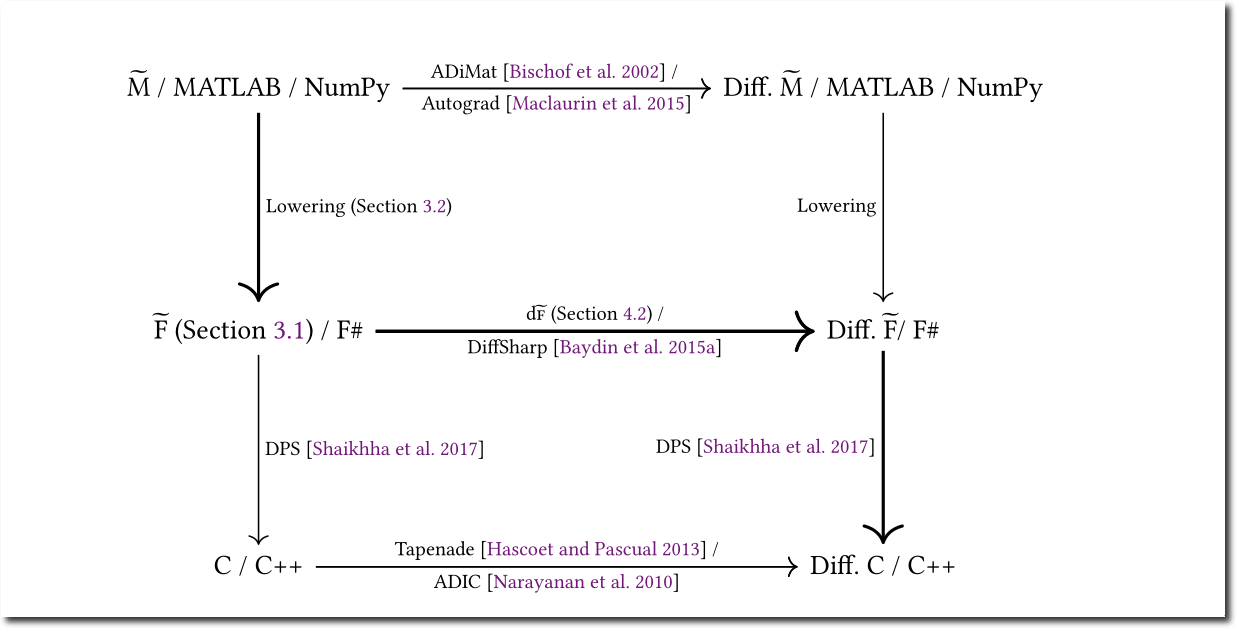
\includegraphics[width=.9\linewidth]{pipeline.png}
\end{center}
\end{frame}


\begin{frame}{d f-smooth and M-smooth}

  \begin{itemize}
    \item The highest level /api/ mimicks the conventional
      interfaces to high level linear algebra libraries and
      languages such as MatLab and Numpy

    \item The program is then lowered into its representation in
      f smooth which computes the actual derivatives. After this computation
      many optimizations can be applied before...

    \item  Compiling once again to C code, where memory is managed in a
      stack like manner by using the destination passing style technique,
      which is just a fancy way to say that the caller is responsible for
      the callees memory and passes to it the memory location where it can
      store the results.

  \end{itemize}

\end{frame}

\begin{frame}{differentiation in df-smooth }

  \begin{itemize}
    \item source to source transformation based on the \texttt{deriv} construct
    \item everything done at compile time, macro-ish
    \item we can call \texttt{deriv} multiple times to get the derivative with respect
      to a list of free variables.
  \end{itemize}
  \begin{enumerate}
    \item first deriv constructs a lambda with the free variables as input parameters
    \item the produced lambda is passed to the source-to-source differentiation
      operator $ \mathcal D $
  \end{enumerate}

\end{frame}

\begin{frame}{example}
  The derivative of the program \texttt{cos a} is represented
  as $\texttt{snd} ((\mathcal D [[\texttt{fun a -> cos a}]]) (a,1)) $
  which expands to
  \begin{equation*}
    \texttt{snd} ((\mathcal D [[ \texttt{fun a -> cos a}]] (a,1)))
  \end{equation*}

\begin{center}
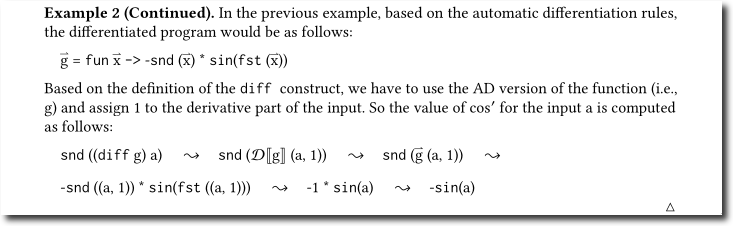
\includegraphics[width=.9\linewidth]{example2.png}
\end{center}

\end{frame}



\begin{frame}{f smooth}

\begin{center}
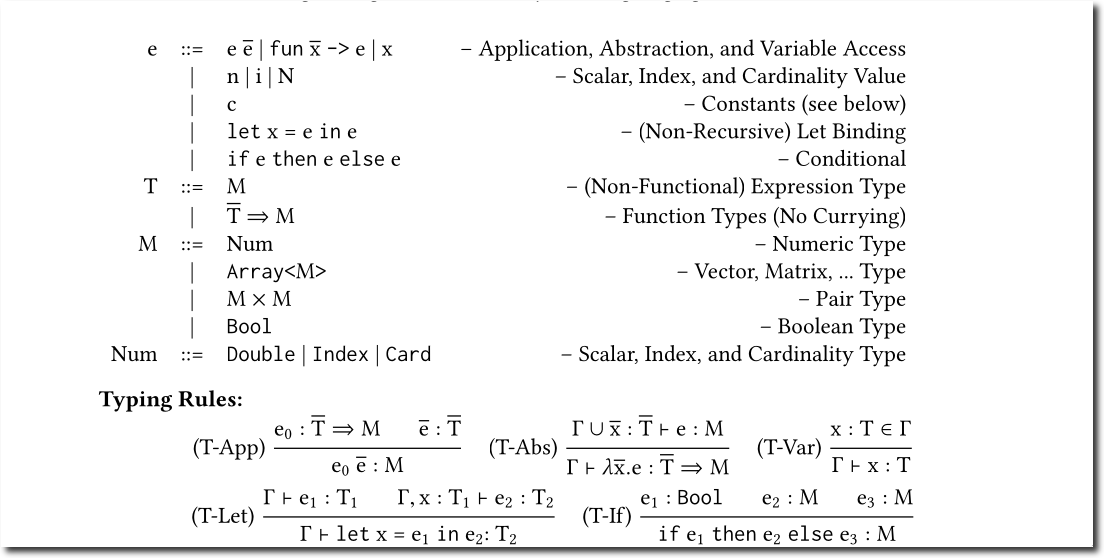
\includegraphics[width=.9\linewidth]{fsmooth1.png}
\end{center}
\end{frame}

\begin{frame}{f smooth 2}

\begin{center}
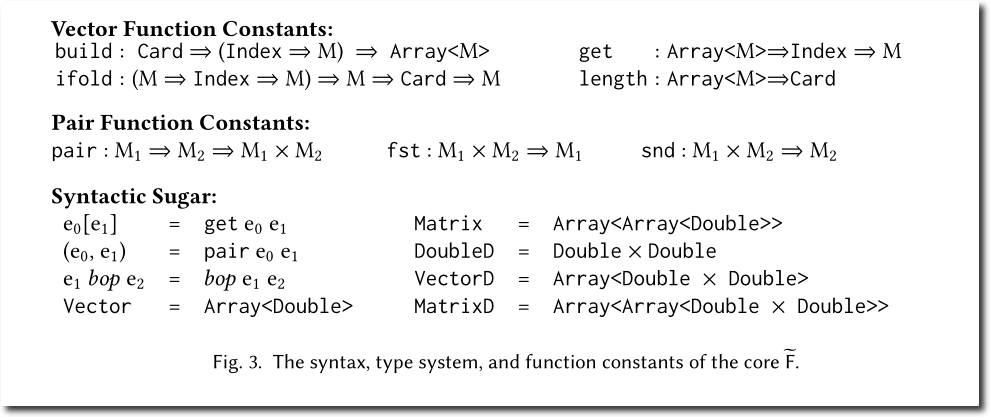
\includegraphics[width=.9\linewidth]{fsmooth2.png}
\end{center}
built in functions for array programming : build ifold and length
\end{frame}



\begin{frame}{loop fusion example}
  In this example we show that taking the tranpose twice of
  a Matrix is the ``same'' as just copying it.
  \begin{center}
    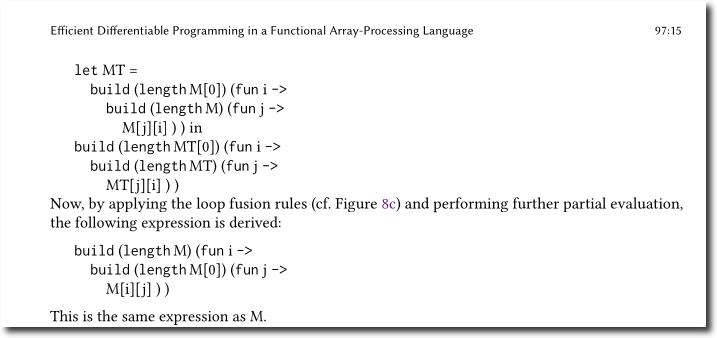
\includegraphics[width=.9\linewidth]{matrixtranspose.png}
  \end{center}
\end{frame}

\end{document}
